\section{存储器层次结构}
\subsection{存储技术}
\subsubsection{随机访问存储器}

\paragraph{SRAM 和 DRAM}
\begin{itemize}
    \item \textbf{静态随机存取存储器}(SRAM, Static Random Access Memory):SRAM 将每个位存储在一个双稳态的 (bistable) 存储器单元里。每个单元由一个六晶体管电路实现。
    \item \textbf{动态随机存取存储器}(DRAM, Dynamic Random Access Memory):DRAM 的每个单元由一个电容和一个访问晶体管组成。它对干扰非常敏感,当电容的电压被扰乱之后,它就永远不会恢复了。
\end{itemize}

只要有供电,SRAM 就会保持不变。与 DRAM 不同,它不需要刷新。SRAM 的存取比 DRAM 快得多。SRAM 对诸如光和电噪声这样的干扰不敏感。代价是 SRAM 单元比 DRAM 单元使用更多的晶体管,因而密度低,而且更贵,功耗更大。
\begin{figure}[H]
    \centering
    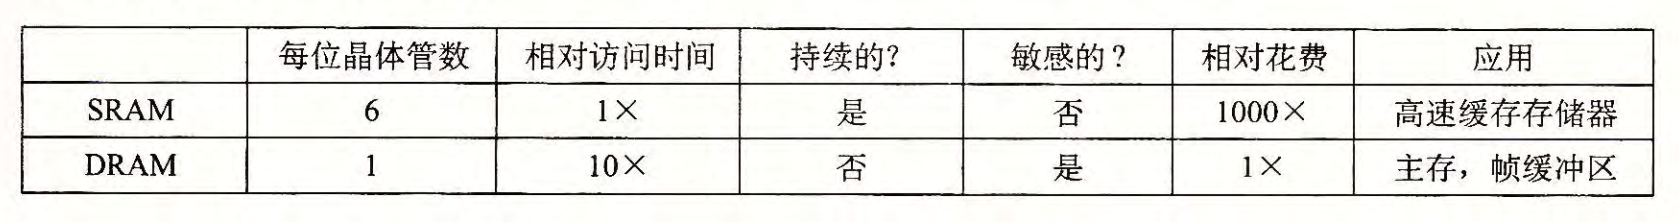
\includegraphics[width=0.8\textwidth]{memory/SRAM-DRAM.png}
\end{figure}

\paragraph{传统的 DRAM}

DRAM 芯片中的单元(位)被分成 d 个超单元 (supercell),每个超单元都由 w 个 DRAM
单元组成。 一个 d×w 的 DRAM 总共存储了 d·w 位信息。超单元被组织成一个 r 行 c 列的长
方形阵列,这里 r c = d。每个超单元有形如 (i,j) 的地址,这里 i 表示行,而 j 表示列。

每个 DRAM 芯片被连接到某个称为内存控制器 (memory controller) 的电路,这个电
路可以一次传送 w 位到每个 DRAM 芯片或一次从每个 DRAM 芯片传出 w 位。为了读出
超单元 (i,j) 的内容,内存控制器将行地址 i 发送到 DRAM,然后是列地址 j。DRAM 把
超单元 (i,j) 的内容发回给控制器作为响应。行地址请求称为 RAS (Row Access Strobe, 行
访问选通脉冲),列地址请求称为 CAS (Column Access Strobe, 列访问选通脉冲)。注意,RAS
和 CAS 请求共享相同的 DRAM 地址引脚。

\begin{figure}[H]
    \centering
    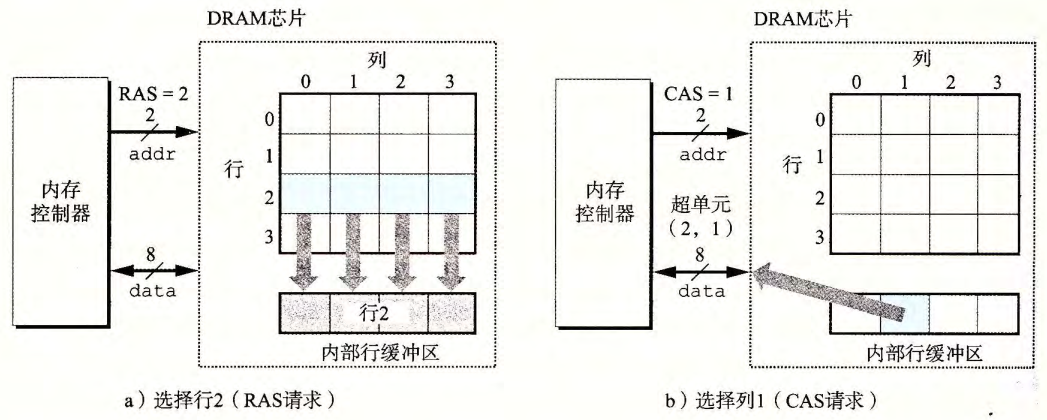
\includegraphics[width=0.8\textwidth]{memory/DRAM-read.png}
\end{figure}

\paragraph{内存模块}
DRAM 芯片封装在内存模块 (memory module) 中,插入到主板的扩展插槽上。
要取出内存地址 A 处的一个字,内存控制器将 A 转换成一个超单元地址 (i, j) 并将
它发送到内存模块,然后内存模块再将 i 和 j 广播到每个 DRAM 芯片。作为响应,每个
DRAM 输出它的 (i, j) 超单元的 8 位内容。模块中的电路收集这些输出,并把它们合并成
一个 64 位字,再返回给内存控制器。
\begin{figure}[H]
    \centering
    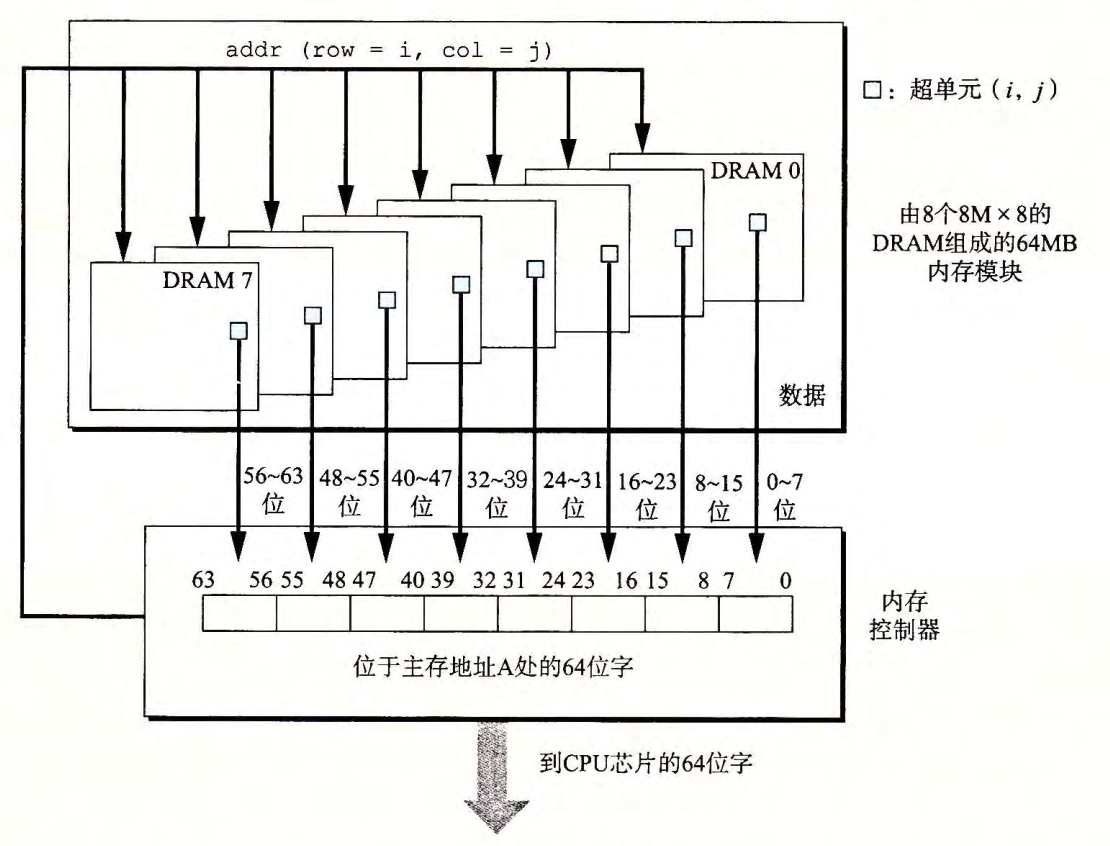
\includegraphics[width=0.8\textwidth]{memory/memory-module.png}
\end{figure}

\paragraph{增强的 DRAM}
\begin{itemize}
    \item 快页模式 DRAM (Fast Page Mode DRAM, FPM DRAM)
    \item 拓展数据输出 DRAM (Extended Data Out DRAM, EDO DRAM)
    \item 同步 DRAM (Synchronous DRAM, SDRAM)
    \item 双数据速率同步 DRAM (Double Data Rate Synchronous DRAM, DDR SDRAM)
    \item 视频 RAM (Video RAM, VRAM)
\end{itemize}

\paragraph{非易失性存储器}
如果断电, DRAM 和 SRAM 会丢失它们的信息,从这个意义上说,它们是易失的
(volatil) 。非易失性存储器 (nonvolatile memory) 即使是在关电后,仍然保存
着它们的信息。
\begin{itemize}
    \item 只读存储器 (Read-Only Memory, ROM)
    \item 可编程只读存储器 (Programmable Read-Only Memory, PROM)
    \item 可擦除可编程只读存储器 (Erasable Programmable Read-Only Memory, EPROM)
    \item 电可擦除可编程只读存储器 (Electrically Erasable Programmable Read-Only Memory, EEPROM)
    \item 闪存 (Flash Memory)
\end{itemize}

\paragraph{访问主存}
数据流通过称为总线 (bus) 的共享电子电路在处理器和 DRAM 主存之间来来回回。每
次 CPU 和主存之间的数据传送都是通过一系列步骤来完成的,这些步骤称为总线事务
(bus transaction) 。读事务 (read transaction) 从主存传送数据到 CPU 。写事务 (write transaction) 从 CPU 传送数据到主存。

下图的主要部件是 CPU 芯片、 I/O
桥接器 (I/O bridge) ,以及组成主存的 DRAM 内存模块。
这些部件由一对总线连接起来,其中一条总线是系统总线 (system bus) , 它连接 CPU 和 
I/O 桥接器,另一条总线是内存总线 (memory bus), 它连接 I/O 桥接器和主存。 I/O 桥接
器将系统总线的电子信号翻译成内存总线的电子信号。 I/O 桥也将
系统总线和内存总线连接到 I/O 总线,像磁盘和图形卡这样的 I/O 设备共享 I/O 总线。

\begin{figure}[H]
    \centering
    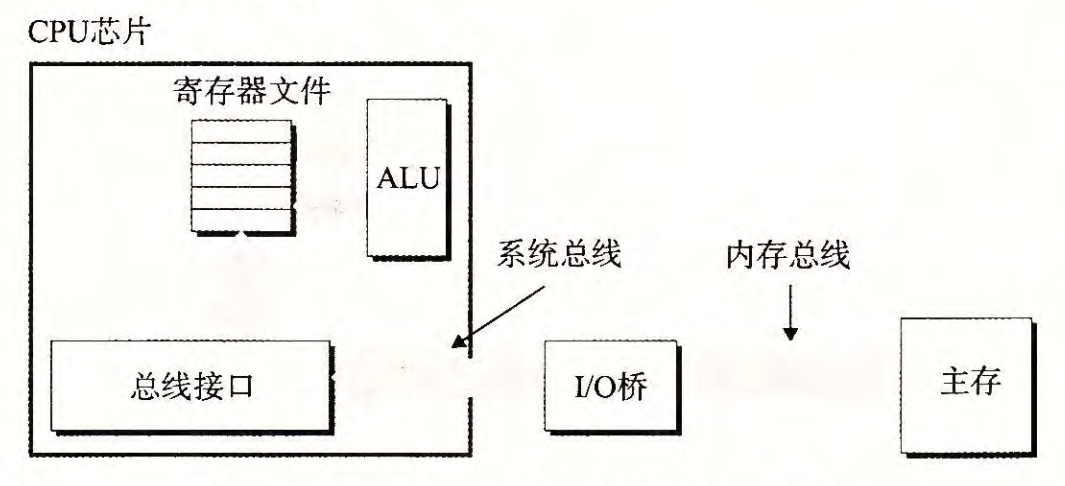
\includegraphics[width=0.8\textwidth]{memory/bus.png}
\end{figure}
\begin{figure}[H]
    \centering
    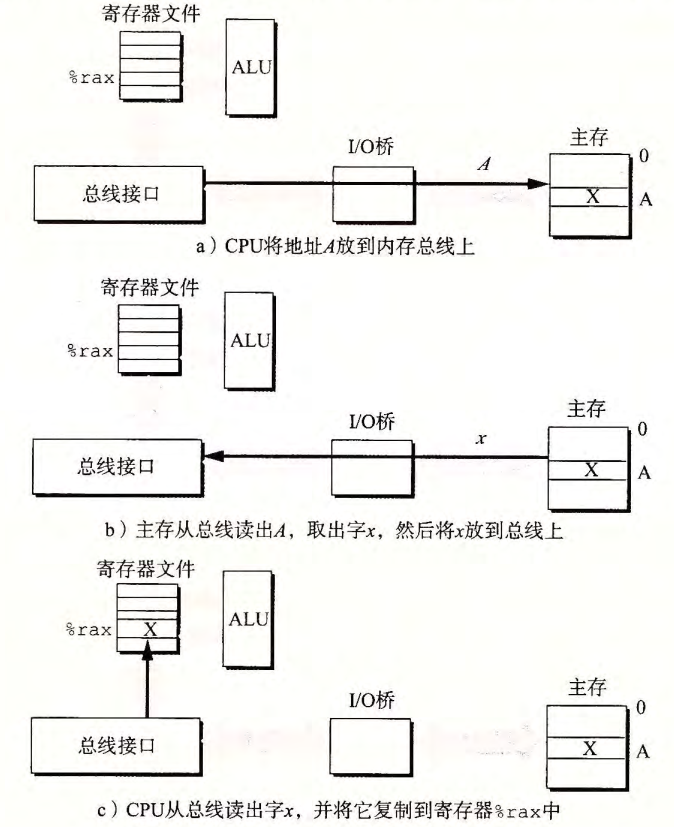
\includegraphics[width=0.8\textwidth]{memory/bus-transaction.png}
\end{figure}

\subsubsection{磁盘存储}
\paragraph{磁盘构造}
磁盘是由盘片 (platter) 构成的。每个盘片有两面,称为表面 (surface),表面覆盖着磁性记录材料。盘片中央有一个可以旋转的主轴 (spindle),它使得盘片以固定的旋转速率 (rotational rate) 旋转,通常是每分钟几千转 (revolutions per minute, RPM)。

每个表面是由一组称为磁道 (track) 的同心圆组成的。每个磁道被划分为一组扇区 (sector)。扇区之间由一些间隙 (gap) 分隔开,这些间隙中不存储数据位,间隙用于存放标识扇区的格式化信息。

磁盘是由一个或多个叠放在一起的盘片组成的,它们被封装在一个密封的包装里,整个装置通常被称为磁盘驱动器 (disk drive),我们通常简称为磁盘 (disk)。

\begin{figure}[H]
    \centering
    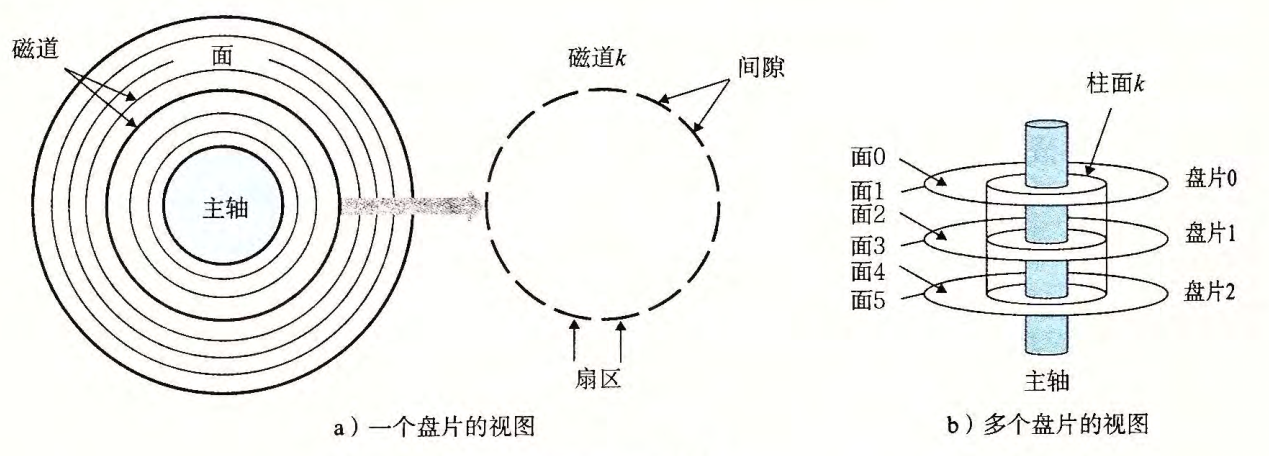
\includegraphics[width=0.8\textwidth]{memory/disk.png}
\end{figure}

\paragraph{磁盘容量}
\begin{itemize}
    \item 记录密度 (recording density):每英寸磁道上的位数。
    \item 轨道密度 (track density):每英寸径向轨道的数量。
    \item 面密度 (areal density):每平方英寸上的位数,记录密度和轨道密度的乘积。
\end{itemize}
\begin{center}
磁盘容量 = 字节数/扇区 $\times$ 平均扇区数/磁道 $\times$ 磁道数/表面 $\times$ 表面数/盘片 $\times$ 盘片数/磁盘
\end{center}
\begin{sidenote}{-千兆字节有多大}
对于与 DRAM 和 SRAM 容量相关的计量单位,通常 $K=2^{10}$,$M=2^{20}$,$G=2^{30}$ 而
$T= 2^{40}$。对于与像磁盘和网络这样的 I/O 设备容量相关的计量单位,通常 $K = 10^{3}$,
$M= 10^{6}$,$G = 10^{9}$,而 $T=10^{12}$。
\end{sidenote}

\paragraph{磁盘操作}

磁盘用读/写头 (read/write head) 来读写存储在磁性表面的位,而读写头连接到一个传动臂 (actuator arm) 一端,通过沿着半径轴前后移动这个传动臂,驱动器可以将读/写头定位在盘面上的任何磁道上。这样的机械运动称为寻道 (seek)。一旦读/写头定位到了期望的磁道上,那么当磁道上的每个位通过它的下面时,读/写头可以感知到这个位的值(读该位),也可以修改这个位的值(写该位)。有多个盘片的磁盘针对每个盘面都有一个独立的读/写头。读/写头垂直排列,一致行动。在任何时刻,所有的读/写头都位于同一个柱面上。

\begin{figure}[H]
    \centering
    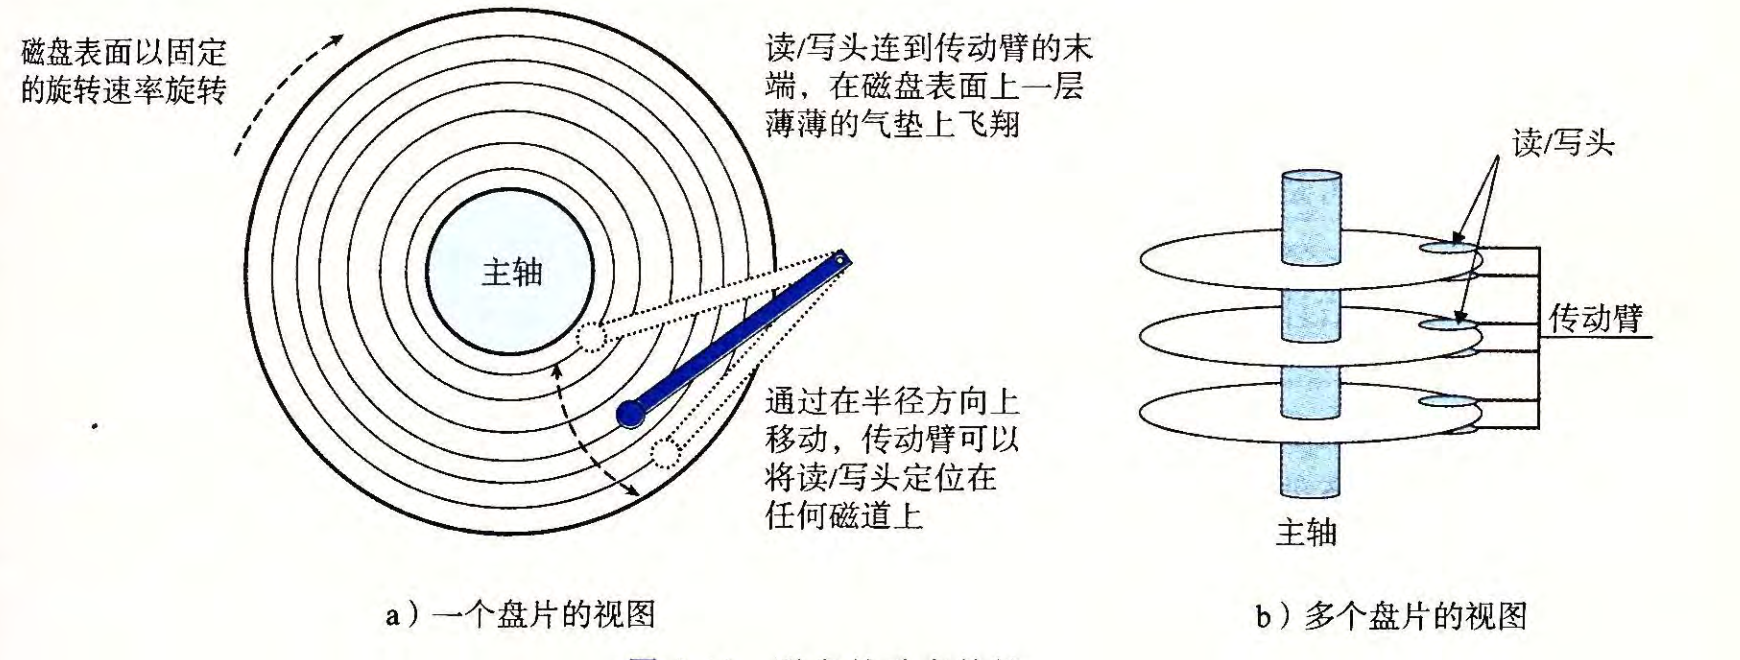
\includegraphics[width=0.8\textwidth]{memory/disk-operation.png}
\end{figure}

对扇区的访问时间 (access time) 有三个主要的部分:
\begin{itemize}
    \item 寻道时间 (seek time):将读/写头移动到正确磁道所需的时间。
    \item 延迟时间 (latency time):等待所需扇区旋转
    \item 传输时间 (transfer time):读写扇区所需的时间。
\end{itemize}

因为寻道时间和旋转延迟大致相等,所以将寻道时间乘 2 是估计磁盘访问时间的简单而合理的方法。

\paragraph{磁盘逻辑块}

\begin{sidenote}{局部性原理}
    局部性原理(Locality Principle)是计算机科学中的一个重要概念,指的是在程序执行过程中,访问的数据和指令往往集中在某些特定的区域。这种现象可以分为两种类型:时间局部性和空间局部性。
    
    \textbf{时间局部性}(Temporal Locality)指的是如果一个数据项在某个时间点被访问,那么在不久的将来它很可能会再次被访问。换句话说,最近使用过的数据很可能会再次被使用。
    
    \textbf{空间局部性}(Spatial Locality)指的是如果一个数据项在某个时间点被访问,那么与它相邻的数据项也很可能会在不久的将来被访问。换句话说,程序倾向于访问存储器中相近的地址。
    
    局部性原理是设计高效存储器层次结构(如缓存、主存和辅助存储器)的基础。通过利用局部性原理,计算机系统可以显著提高数据访问速度,减少延迟,从而提升整体性能。

\end{sidenote}


\subsection{缓存}
